%%%%%%%%%%%%%%%%%%%%%%%%%%%%%%%%%%%%%%%%%
% University/School Laboratory Report
% LaTeX Template
% Version 3.0 (4/2/13)
%
% This template has been downloaded from:
% http://www.LaTeXTemplates.com
%
% Original author:
% Linux and Unix Users Group at Virginia Tech Wiki 
% (https://vtluug.org/wiki/Example_LaTeX_chem_lab_report)
%
% License:
% CC BY-NC-SA 3.0 (http://creativecommons.org/licenses/by-nc-sa/3.0/)
%
%%%%%%%%%%%%%%%%%%%%%%%%%%%%%%%%%%%%%%%%%

%----------------------------------------------------------------------------------------
%	PACKAGES AND DOCUMENT CONFIGURATIONS
%----------------------------------------------------------------------------------------

\documentclass{article}

\usepackage[version=3]{mhchem} % Package for chemical equation typesetting
\usepackage{siunitx} % Provides the \SI{}{} command for typesetting SI units

\usepackage{graphicx}
\usepackage{caption}
\usepackage{subcaption}
\usepackage{cancel}

\usepackage{float}

\usepackage[T1]{fontenc} % allow small bold caps

\setlength\parindent{0pt} % Removes all indentation from paragraphs

\renewcommand{\labelenumi}{\alph{enumi}.} % Make numbering in the enumerate environment by letter rather than number (e.g. section 6)

\usepackage[margin=1in]{geometry}

\usepackage{amssymb}

%\usepackage{times} % Uncomment to use the Times New Roman font

%----------------------------------------------------------------------------------------
%	Title
%----------------------------------------------------------------------------------------

\begin{document}
\pagenumbering{gobble}

\title{6.s02: EECS II - From A Medical Perspective}
\author{
  Ryan Lacey <rlacey@mit.edu>\\
  \footnotesize \texttt{Collaborator(s): Jorge Perez}
}
        
\maketitle
        


\begin{enumerate}

\item[1.]
	\begin{enumerate}
	\item[(a)] 
		        Analytical expression for DT signal $x_1[n]$\\
		        
		        $x_1[n] = \cos{\left(\omega n\right)}$\\
		        
		        $\cos{\left(16\omega\right)} = 1$\\
		        $16\omega = 2\pi$\\
		        $\omega = \frac{\pi}{8}$\\
		        
		        $x_1[n] = \cos{\left( \frac{\pi}{8} n \right)}$
\bigskip
	\item[(b)] 
		        Sampling Frequency (Hz)\\
		        \newline
		        $\omega = 2\pi f$\\
		        $f = \frac{\omega}{2\pi} = \frac{\frac{\pi}{8}}{2\pi} = \frac{1}{16}$
\bigskip
	\item[(c)] 
		        Analytical form of CT signal that corresponds to $x_1[n]$\\
		        \newline
		        $x(t) = \cos{\left( \omega n T s \right)} = \cos{\left( \omega T \right)}$\\
		        
		        $x(16) = \cos{\left( \omega (16)(5) \right)} = 1$\\
		        $\omega (16)(5) = 2\pi$\\
		        $\Omega = \frac{\pi}{40}$\\
		        
		        $x(t) = \cos{\left( \frac{\pi}{40} T \right)}$
\bigskip
	\item[(d)] 
		        Analytical form of CT signal with sampling frequency decreased by 2\\
		        \newline
		        $T$ is doubled\\
		        $\omega (16)(5 \times 2) = 2\pi$\\
		        $\Omega = \frac{\pi}{80}$\\
		        
		        $x(t) = \cos{\left( \frac{\pi}{80} T \right)}$
	\end{enumerate}

\newpage

\item[2.]
	\begin{enumerate}
	\item[(a)] 
		        Minimum interval between heartbeats, in samples, determined by minimum distance between peaks: $\texttt{213 \text{samples/beat}}$
\bigskip
	\item[(b)] 
		        Sampling Rate\\
		        \newline
		        $\frac{\texttt{101.483 \text{beat}}}{\texttt{1 \cancel{\text{min}}}} \cdot  \frac{\texttt{1 \cancel{\text{min}}}}{\texttt{60 \text{sec}}} = \texttt{1.694 \text{beats/sec}}$\\
		        \newline
		        $\frac{\texttt{1.691 \cancel{\text{beat}}}}{\texttt{1 \text{sec}}} \cdot  \frac{\texttt{213 \text{sample}}}{\texttt{1 \cancel{\text{beat}}}} \approx \texttt{360 \text{sample/sec}}$
\bigskip
	\item[(c)] 
		        Total Beats\\
		        \newline
		        $\texttt{20500 \cancel{\text{sample}}} \cdot  \frac{\texttt{1 {\text{beat}}}}{\texttt{213 \cancel{\text{sample}}}} = \texttt{96.24 \text{beats}}$
\bigskip
	\item[(d)] 
		        x-axis: \texttt{Time (sec)}\\
		        y-axis: \texttt{ABP (mmHg)}\\
		        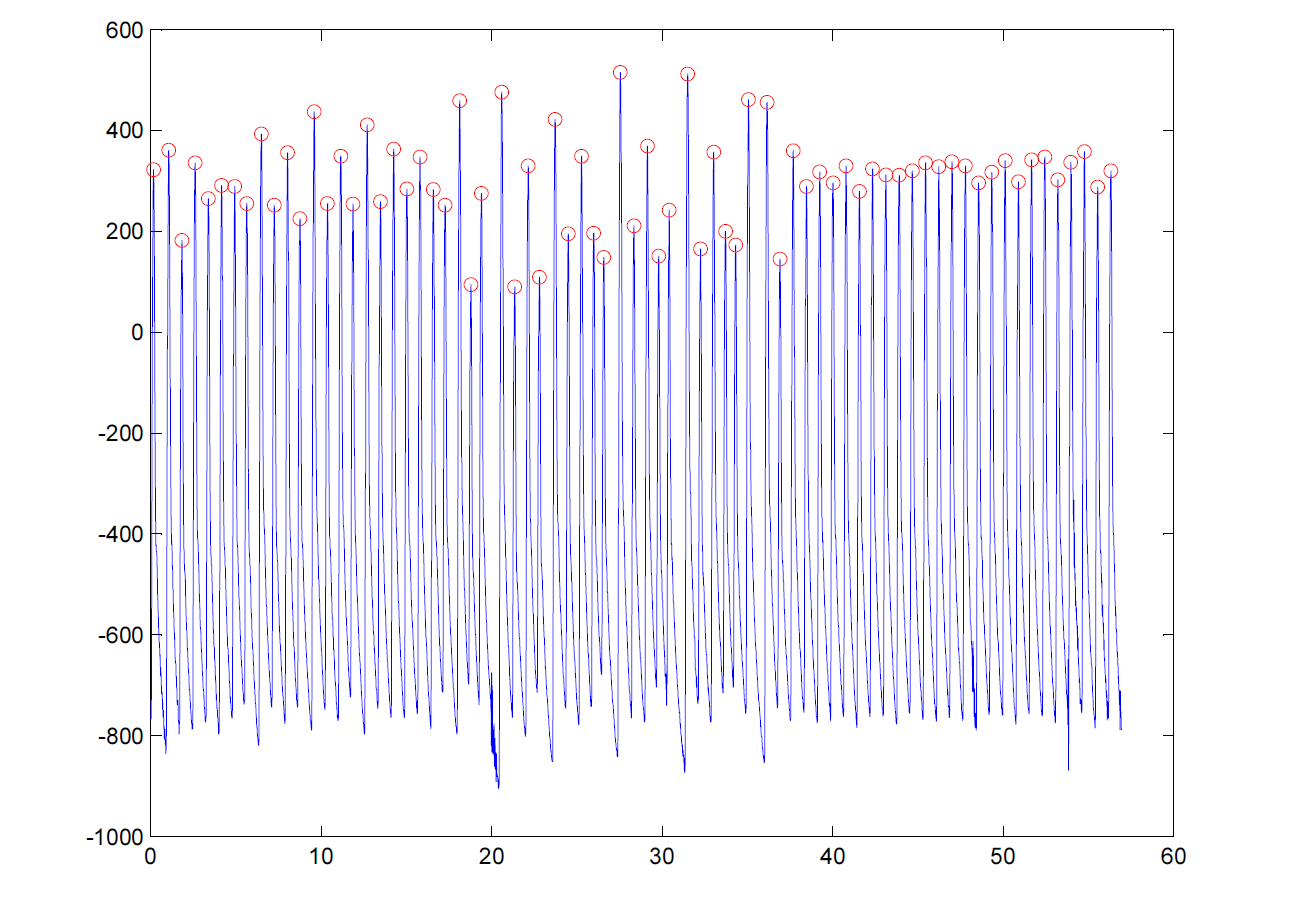
\includegraphics[width=\linewidth]{2dpeaks} 
	\end{enumerate}

\newpage

\item[3.]
	\begin{enumerate}
	\item[(a)] 
		        $I(1) = -\dfrac{2nFADC_0}{L} e^{\frac{-\pi^2Dt}{4L^2}}$ \\
		        
		        $I(2) = -\dfrac{2nFADC_0}{L} e^{\frac{-9\pi^2Dt}{4L^2}}$ \\
		        \newline\newline
		        $\dfrac{I(2)}{I(1)} = \dfrac{-\dfrac{2nFADC_0}{L} e^{\frac{-9\pi^2Dt}{4L^2}}}{-\dfrac{2nFADC_0}{L} e^{\frac{-\pi^2Dt}{4L^2}}} = e^{\frac{-8\pi^2Dt}{4L^2}}$ \\
\bigskip
	\item[(b)] 
		        $0.01 = e^{\frac{-8\pi^2Dt}{4L^2}}$ \\
		        
		        $t = - \ln{\left(0.01 \frac{4L^2}{8 \pi^2 D}\right)}$
\bigskip
	\item[(c)] 
		        $t = - \ln{\left(0.01 \frac{4(50 \times 10^{-6})^2}{8 \pi^2 (6 \times 10^{-10})}\right)} = 6.16$
\bigskip
	\item[(d)] Estimate of current for $t > T_{0.01}$\\
		        
		        $I_{bar}(t) = -\dfrac{2nFADC_0}{L} e^{\frac{-\pi^2Dt}{4L^2}}$ \\
	\end{enumerate}

\newpage

\item[4.]
	\begin{enumerate}
	\item[(a)] 
		        $C_0 = \frac{\texttt{1 \text{mol}}}{\texttt{180.16 \cancel{\text{g}}}} \cdot \frac{\texttt{1 \cancel{\text{g}}}}{\texttt{1000 \cancel{\text{mg}}}} \cdot  \frac{\texttt{320 \cancel{\text{mg}}}}{\texttt{1 \cancel{\text{dL}}}} \cdot \frac{\texttt{10 \cancel{\text{dL}}}}{\texttt{1 \text{L}}} = \texttt{0.0178 \text{mol/L}}$
\bigskip
	\item[(b)] 
		        x-axis: \texttt{Time (sec)}\\
		        y-axis: \texttt{Log Current (amp)}\\
		        $\Delta$: 5.1 second delay\\
		        $D$: $2.1 \times 10^{-10}$ $m^2/s$\\
		        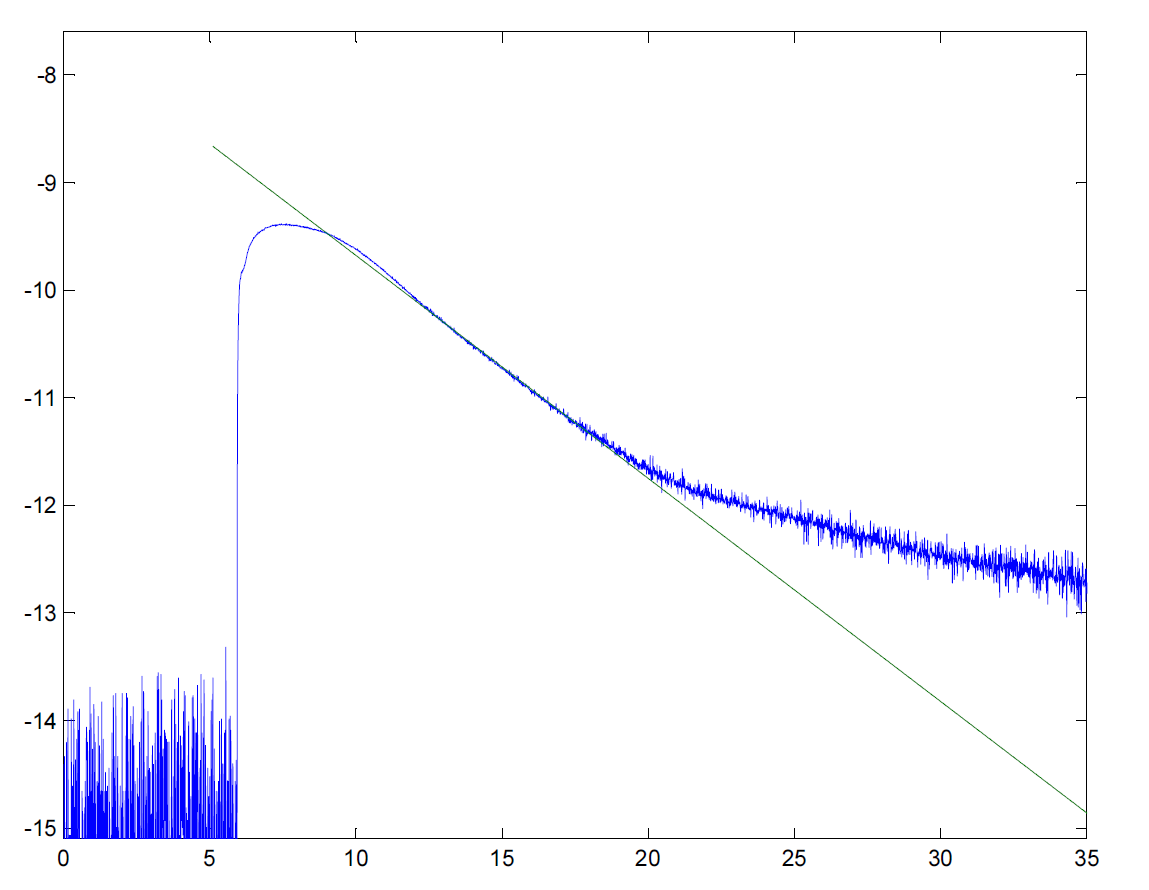
\includegraphics[width=\linewidth]{decay} 
\bigskip
	\item[(c)] 
		        $T_2$ = 24.42 seconds\
		        
		        Found by iterating through time for $t>10$ (this is approximately when we enter the exponential portion of the graph) and searching for the first time $t$ at which the difference between the actual data and the line of best fit is greater than 1.
	\end{enumerate}


\end{enumerate}

\end{document}